% ============================================================
% defense_presentation.tex
% Active Management Puzzle — PhD Defense
% Ömer Eren | Boğaziçi University, Management Department
% Supervisor: Prof. Vedat Akgiray | June 2026
%
% Engine: XeLaTeX
% Theme:  Beamer metropolis
% ============================================================

\documentclass[10pt, aspectratio=169]{beamer}

% ---------- Theme -------------------------------------------
\usetheme[progressbar=frametitle, block=fill]{metropolis}
\setbeamertemplate{navigation symbols}{}

% ---------- Packages ----------------------------------------
\usepackage{fontspec}
\usepackage{amsmath, amssymb}
\usepackage{booktabs}
\usepackage{graphicx}
\usepackage{xcolor}
\usepackage{tikz}
\usetikzlibrary{positioning, arrows.meta, decorations.pathreplacing, calligraphy}
\usepackage{array}
\usepackage{multirow}
\usepackage{colortbl}
\usepackage[style=apa, backend=biber]{biblatex}
\addbibresource{dissertation.bib}
\usepackage{appendixnumberbeamer}

% ---------- Colors ------------------------------------------
\definecolor{mDarkTeal}{HTML}{23373b}
\definecolor{mMidTeal}{HTML}{3d7a84}
\definecolor{mLightGray}{HTML}{f5f5f5}
\definecolor{alertred}{HTML}{b71c1c}
\definecolor{successgreen}{HTML}{1b5e20}
\definecolor{warningyellow}{HTML}{f57f17}
\definecolor{neutralblue}{HTML}{0d47a1}

% Redefine alerted text colour
\setbeamercolor{alerted text}{fg=alertred}

% ---------- Custom commands ---------------------------------
\newcommand{\yes}{\textcolor{successgreen}{\textbf{Confirmed}}}
\newcommand{\no}{\textcolor{alertred}{\textbf{Not confirmed}}}
\newcommand{\bp}{\,\text{bp}}
\newcommand{\pct}{\%}
\newcommand{\source}[1]{\vspace{2pt}\begin{flushright}\tiny\textit{#1}\end{flushright}}

% ---------- Frametitle strut --------------------------------
\makeatletter
\setlength{\metropolis@frametitle@padding}{2.2ex}
\makeatother

% ============================================================
\title{Active Management:\\[4pt]
       \normalsize Informational Necessity or Psychological Utility?}
\subtitle{Investigating the Behavioral Drivers of the Active Management Puzzle}
\author{Ömer Eren}
\institute{%
  Department of Management, Boğaziçi University\\[2pt]
  Supervisor: Prof.\ Vedat Akgiray}
\date{June 2026}

% ============================================================
\begin{document}

% ---- Title slide -------------------------------------------
{%
\setbeamertemplate{footline}{}
\begin{frame}
  \titlepage
  \vfill
  \footnotesize
  \begin{tabular}{@{}ll}
    Jury: & Prof.\ V.\ Akgiray \textbar{} Assoc.\ Prof.\ A.\ Coşkun \textbar{}
            Assoc.\ Prof.\ C.C.\ Karahan \\
          & Assist.\ Prof.\ E.\ Ahi \textbar{} Assist.\ Prof.\ H.\ Özsöylev
  \end{tabular}
\end{frame}
}

% ---- Roadmap -----------------------------------------------
\begin{frame}{Roadmap}
\setlength{\tabcolsep}{6pt}
\footnotesize
\begin{tabular}{@{}cl@{\hspace{12pt}}cl}
  \textbf{I}   & Motivation \& Research Question  &
  \textbf{VIII}& H1: Sentiment-Convexity \\
  \textbf{II}  & Data \& Sample Construction      &
  \textbf{IX}  & H2: Disposition / Illusion of Control \\
  \textbf{III} & Aggregate Performance            &
  \textbf{X}   & H3: Lottery Demand \\
  \textbf{IV}  & Bootstrap \& FDR Decomposition  &
  \textbf{XI}  & H4: Fee Elasticity \\
  \textbf{V}   & Structural Break \& Sub-Periods  &
  \textbf{XII} & Psychological Premium Framework \\
  \textbf{VI}  & Activeness \& Persistence        &
  \textbf{XIII}& Discussion \& Synthesis \\
  \textbf{VII} & Behavioral Framework             &
  \textbf{XIV} & Conclusion \\
\end{tabular}
\end{frame}

% ============================================================
%  PART I — MOTIVATION
% ============================================================
\section{I.\ Motivation \& Research Question}

\begin{frame}{Sharpe's Arithmetic \& Gruber's Puzzle}
  \begin{columns}[T]
    \begin{column}{0.48\textwidth}
      \textbf{The tautology (Sharpe 1991)}
      \begin{itemize}\itemsep4pt
        \item Before costs, the average active dollar \emph{must} match the market.
        \item After costs, the average active dollar \emph{must} underperform.
        \item \alert{Not an empirical claim — it is arithmetic.}
      \end{itemize}
      \vspace{6pt}
      \textbf{Three decades of evidence}
      \begin{itemize}\itemsep4pt
        \item Jensen (1968), Carhart (1997), Fama \& French (2010): active funds
              deliver negative net alpha on average.
        \item Barras, Scaillet \& Wermers (2010): the fraction of genuinely skilled
              managers is negligible.
      \end{itemize}
    \end{column}
    \begin{column}{0.48\textwidth}
      \textbf{Yet the puzzle persists (Gruber 1996)}
      \begin{itemize}\itemsep4pt
        \item US active equity mutual funds still hold $>$\$10 trillion in AUM.
        \item Capital inflows are structurally positive in most years.
        \item Flow–performance convexity (Sirri \& Tufano 1998) is intact.
      \end{itemize}
      \vspace{6pt}
      \begin{block}{The Active Management Puzzle}
        Why do rational investors persistently allocate to
        strategies that underperform passive alternatives net of fees?
      \end{block}
    \end{column}
  \end{columns}
\end{frame}

\begin{frame}{Two Competing Explanations}
  \begin{columns}[T]
    \begin{column}{0.48\textwidth}
      \begin{block}{Rational Equilibrium}
        \textbf{Berk \& Green (2004)}
        \begin{itemize}\itemsep4pt
          \item Skilled managers exist; rational investors chase them.
          \item Capital inflows erode skill advantages (decreasing returns to scale).
          \item Equilibrium: net alpha $\approx 0$ in value-weighted terms.
          \item Puzzle is an artefact of equal-weighting.
        \end{itemize}
      \end{block}
    \end{column}
    \begin{column}{0.48\textwidth}
      \begin{block}{Behavioral Frictions}
        \textbf{Four channels tested here}
        \begin{itemize}\itemsep4pt
          \item \textbf{H1} Sentiment amplifies winner-chasing.
          \item \textbf{H2} Margin pressure locks in losers.
          \item \textbf{H3} Lottery appeal weakens exit discipline.
          \item \textbf{H4} Fee sensitivity relaxes under optimism.
        \end{itemize}
        If any channel is operative, flows contain a behavioral
        component not explained by rational updating.
      \end{block}
    \end{column}
  \end{columns}
\end{frame}

\begin{frame}{Research Question \& Scope}
  \metroset{block=transparent}
  \begin{block}{\large Central Question}
    \centering
    Does investor persistence in active funds reflect the\\
    \textbf{rational equilibrium of Berk \& Green (2004)},\\
    or does it require \textbf{behavioral explanations}?
  \end{block}
  \vspace{10pt}
  \begin{columns}[T]
    \begin{column}{0.3\textwidth}
      \textbf{Universe}\\
      3,764 US domestic equity mutual fund share classes\\
      (one primary per fund)
    \end{column}
    \begin{column}{0.3\textwidth}
      \textbf{Period}\\
      December 1994 –\\
      February 2026\\
      (373 months)
    \end{column}
    \begin{column}{0.3\textwidth}
      \textbf{Data}\\
      Bloomberg Terminal\\ + LSEG Workspace\\
      (Boğaziçi Dept.\ subscriptions)
    \end{column}
  \end{columns}
\end{frame}

\begin{frame}{Five Analytical Pillars}
  \begin{tikzpicture}[
      box/.style={draw=mDarkTeal, fill=mLightGray, rounded corners=3pt,
                  text width=2.7cm, align=center, minimum height=1.6cm,
                  font=\footnotesize},
      arr/.style={-{Stealth[length=4pt]}, thick, mMidTeal}
    ]
    \node[box] (a) at (0,0)      {\textbf{Alpha}\\\textbf{Estimation}\\Carhart (1997)\\Newey–West};
    \node[box] (b) at (3.2,0)    {\textbf{Bootstrap}\\\textbf{\& FDR}\\FF (2010)\\BSW (2010)};
    \node[box] (c) at (6.4,0)    {\textbf{Structural}\\\textbf{Break}\\Bai–Perron\\Sub-periods};
    \node[box] (d) at (9.6,0)    {\textbf{Activeness}\\\textbf{\& Persistence}\\$1-R^2$, TE\\KTWW (2006)};
    \node[box] (e) at (12.8,0)   {\textbf{Behavioral}\\\textbf{Panel}\\H1–H4\\PPF};
    \draw[arr] (a) -- (b);
    \draw[arr] (b) -- (c);
    \draw[arr] (c) -- (d);
    \draw[arr] (d) -- (e);
  \end{tikzpicture}
\end{frame}

% ============================================================
%  PART II — DATA
% ============================================================
\section{II.\ Data \& Sample Construction}

\begin{frame}{Universe Construction}
  \begin{columns}[T]
    \begin{column}{0.55\textwidth}
      \textbf{Bloomberg pull}
      \begin{itemize}\itemsep3pt
        \item 2,786 share classes with monthly returns, TNA, expense ratios.
        \item Active/Passive classification: \texttt{Actively\_Managed} field.
        \item LSEG Workspace: Lipper category codes + benchmark total-return series.
        \item 97 active funds: benchmark confirmed via SEC filings and prospectuses.
      \end{itemize}
      \vspace{6pt}
      \textbf{One-share-class-per-fund rule}\\
      Largest share class by time-series length selected as primary;
      prevents within-fund double-counting in all analyses.
    \end{column}
    \begin{column}{0.42\textwidth}
      \footnotesize
      \begin{tabular}{lrrrr}
        \toprule
        Panel & Active & Passive & Unk. & Total \\
        \midrule
        Master           & 2,316 & 342 & 1,033 & 3,691 \\
        Incub.-Corrected & 2,172 & 308 &   742 & 3,222 \\
        Trimmed 1995–23  & 2,082 & 302 &   742 & 3,126 \\
        \bottomrule
      \end{tabular}
      \vspace{4pt}\\
      \tiny Analytical samples after Entire-Analysis exclusions\\
      (leveraged, sector-only, long/short, data-error flags):\\
      3,581 / 3,138 / 3,046 respectively.
    \end{column}
  \end{columns}
\end{frame}

\begin{frame}{Lipper Classification \& Three-Tier Exclusion Scheme}
  \begin{columns}[T]
    \begin{column}{0.50\textwidth}
      \textbf{Lipper classification}
      \begin{itemize}\itemsep3pt
        \item 22 US domestic equity Lipper categories.
        \item Used for within-category performance ranking in H1–H4 panel.
        \item Funds ranked monthly within category (Hodges–Lehmann fractional rank).
      \end{itemize}
      \vspace{6pt}
      \textbf{Incubation bias (Evans 2010)}\\
      First 36 months of each fund's history dropped.\\
      \texttt{panel\_incubation}: no date cap.\\
      \texttt{panel\_trimmed}: additionally capped at 1995–2023
      (used for H1–H4 behavioral regressions where sentiment series ends Dec 2023).
    \end{column}
    \begin{column}{0.46\textwidth}
      \textbf{Flagged exclusion ledger}
      \vspace{4pt}\\
      \footnotesize
      \begin{tabular}{@{}lp{5cm}@{}}
        \toprule
        Flag & Scope \\
        \midrule
        \texttt{excluded\_all}  & Dropped from all analyses (leveraged, sector-only, bear-market, data errors) \\
        \texttt{excluded\_perf} & Dropped from performance comparison only (benchmark mismatch, <24 obs) \\
        \texttt{excluded\_h3}   & Dropped from H3/activeness (covered-call overlays, sector mandates) \\
        \bottomrule
      \end{tabular}
    \end{column}
  \end{columns}
\end{frame}

\begin{frame}{Sample Timeline \& Sub-Period Structure}
  \begin{tikzpicture}[x=0.065\textwidth, y=1cm]
    % Main timeline bar
    \fill[mLightGray!80, draw=mDarkTeal, line width=0.8pt]
      (0,0) rectangle (15.4, 0.7);
    % Sub-period colours
    \fill[neutralblue!25] (0,0)      rectangle (5.33, 0.7);   % P1
    \fill[successgreen!25] (5.33,0)  rectangle (8.57, 0.7);   % P2
    \fill[alertred!20]    (8.57,0)   rectangle (15.4, 0.7);   % P3
    % Labels inside bars
    \node[font=\scriptsize\bfseries] at (2.67, 0.35) {P1};
    \node[font=\scriptsize\bfseries] at (6.95, 0.35) {P2};
    \node[font=\scriptsize\bfseries] at (12.0, 0.35) {P3};
    % Boundary verticals
    \draw[mDarkTeal, dashed, line width=0.8pt] (5.33,-0.4) -- (5.33, 1.1);
    \draw[mDarkTeal, dashed, line width=0.8pt] (8.57,-0.4) -- (8.57, 1.1);
    % Tick labels bottom
    \foreach \x/\lbl in {0/Dec 1994, 5.33/Dec 2005, 8.57/Sep 2011, 15.4/Feb 2026}
      \node[font=\tiny, below] at (\x, 0) {\lbl};
    % Period labels above
    \node[font=\tiny, above] at (2.67, 0.7)
      {\textcolor{neutralblue}{P1: 132 months}};
    \node[font=\tiny, above] at (6.95, 0.7)
      {\textcolor{successgreen}{P2: 69 months}};
    \node[font=\tiny, above] at (12.0, 0.7)
      {\textcolor{alertred}{P3: 173 months}};
    % Key events
    \draw[warningyellow, thick, ->] (1.8, -1.2) -- (1.8, -0.1)
      node[font=\tiny, below=10pt, align=center] {Dot-com\\peak};
    \draw[warningyellow, thick, ->] (5.8, -1.2) -- (5.8, -0.1)
      node[font=\tiny, below=10pt, align=center] {GFC};
    \draw[alertred, thick, ->]    (8.57,-1.2) -- (8.57,-0.1)
      node[font=\tiny, below=10pt, align=center] {\textbf{Break}\\Nov 2011};
    \draw[warningyellow, thick, ->] (12.5,-1.2) -- (12.5,-0.1)
      node[font=\tiny, below=10pt, align=center] {COVID};
  \end{tikzpicture}
  \vspace{10pt}\\
  \footnotesize Break dates from Bai–Perron (1998, 2003) test on rolling Carhart gross alpha.
  Three-regime partition adopted: P1 ($+0.09\pct$ p.a.), P2 ($+0.74\pct$), P3 ($-1.36\pct$).
\end{frame}

\begin{frame}{Descriptive Statistics: Key Moments}
  \footnotesize
  \begin{tabular}{lrrrrrr}
    \toprule
    & $N$ & Fund-months & Mean ret. & VW Mean & Median & SD \\
    \midrule
    Active (Incub.-Corr.) & 2,172 & 425,622 & 0.900 & 0.848 & 1.255 & 4.983 \\
    Passive (Incub.-Corr.)& 308   & 51,422  & 0.918 & 1.015 & 1.365 & 5.006 \\
    \bottomrule
  \end{tabular}
  \vspace{8pt}
  \begin{itemize}\itemsep4pt
    \item Monthly gross returns (\%). Active and passive funds track closely in raw returns.
    \item The underperformance story lives entirely in \textbf{net returns after fees}.
    \item Active mean expense ratio $\approx 1.06\pct$ p.a.; passive $\approx 0.24\pct$ p.a.
    \item Performance-comparison subsample (perf flag): \textbf{1,973 active}, \textbf{281 passive}.
  \end{itemize}
\end{frame}

% ============================================================
%  PART III — AGGREGATE PERFORMANCE
% ============================================================
\section{III.\ Aggregate Performance}

\begin{frame}{Carhart (1997) Four-Factor Model}
  \[
    R_{i,t} - R_{f,t} \;=\; \alpha_i + \beta_i \,\text{MKT}_t
                            + s_i \,\text{SMB}_t
                            + h_i \,\text{HML}_t
                            + p_i \,\text{MOM}_t
                            + \varepsilon_{i,t}
  \]
  \begin{itemize}\itemsep5pt
    \item Time-series regression; alpha annualised ($\times 12$).
    \item \textbf{Newey–West HAC} standard errors (6-month lag) throughout.
    \item Portfolio-level estimation (EW and VW aggregate portfolio series).
    \item Net returns: gross less $\text{ER}/12$ each month (Carhart 1997, Wermers 2000).
    \item Symmetry requirement: bootstrap simulated $t$-stats use \emph{same} NW lag as actual.
  \end{itemize}
\end{frame}

\begin{frame}{Headline Result: Aggregate Net Alpha}
  \footnotesize
  \begin{columns}[T]
    \begin{column}{0.52\textwidth}
      \begin{tabular}{lrrrrrr}
        \toprule
        & $N$ & $T$ & \multicolumn{2}{c}{Gross $\alpha$} & \multicolumn{2}{c}{Net $\alpha$} \\
        \cmidrule(l){4-5}\cmidrule(l){6-7}
        & & & EW & VW & EW & VW \\
        \midrule
        Active  & 1,973 & 373 & $-0.29$ & $-0.19$ & $\mathbf{-1.36}^{***}$ & $\mathbf{-0.90}^{**}$ \\
                & & & $(-0.65)$ & $(-0.49)$ & $(-3.11)$ & $(-2.35)$ \\[2pt]
        Passive & 281   & 373 & $-0.29$ & $0.16$  & $-0.81^{**}$ & $0.02$ \\
                & & & $(-0.82)$ & $(0.69)$  & $(-2.34)$ & $(0.11)$ \\
        \bottomrule
      \end{tabular}
      \vspace{4pt}\\
      \tiny Carhart four-factor alpha (\%, annualised). NW $t$-stats in parentheses.
      $^{**}p<0.05$, $^{***}p<0.01$.
    \end{column}
    \begin{column}{0.45\textwidth}
      \textbf{Key takeaways}
      \begin{itemize}\itemsep5pt
        \item EW net $\alpha = -1.361\pct$: statistically and economically significant.
        \item VW net $\alpha = -0.900\pct$: significant but smaller.
        \item \textbf{VW gap vs.\ passive}: $-0.90 - 0.02 = -92\bp$ p.a.
        \item Gross alpha near zero → underperformance is driven by \alert{fees}, not stock-selection failure.
        \item \textbf{BG prediction: VW $\approx 0$?} At $-0.90\pct$, the evidence is mixed.
      \end{itemize}
    \end{column}
  \end{columns}
\end{frame}

\begin{frame}{Rolling Alpha (Figure 2)}
  \begin{columns}[T]
    \begin{column}{0.55\textwidth}
      \IfFileExists{tables/fig_rolling_alphas.png}{%
        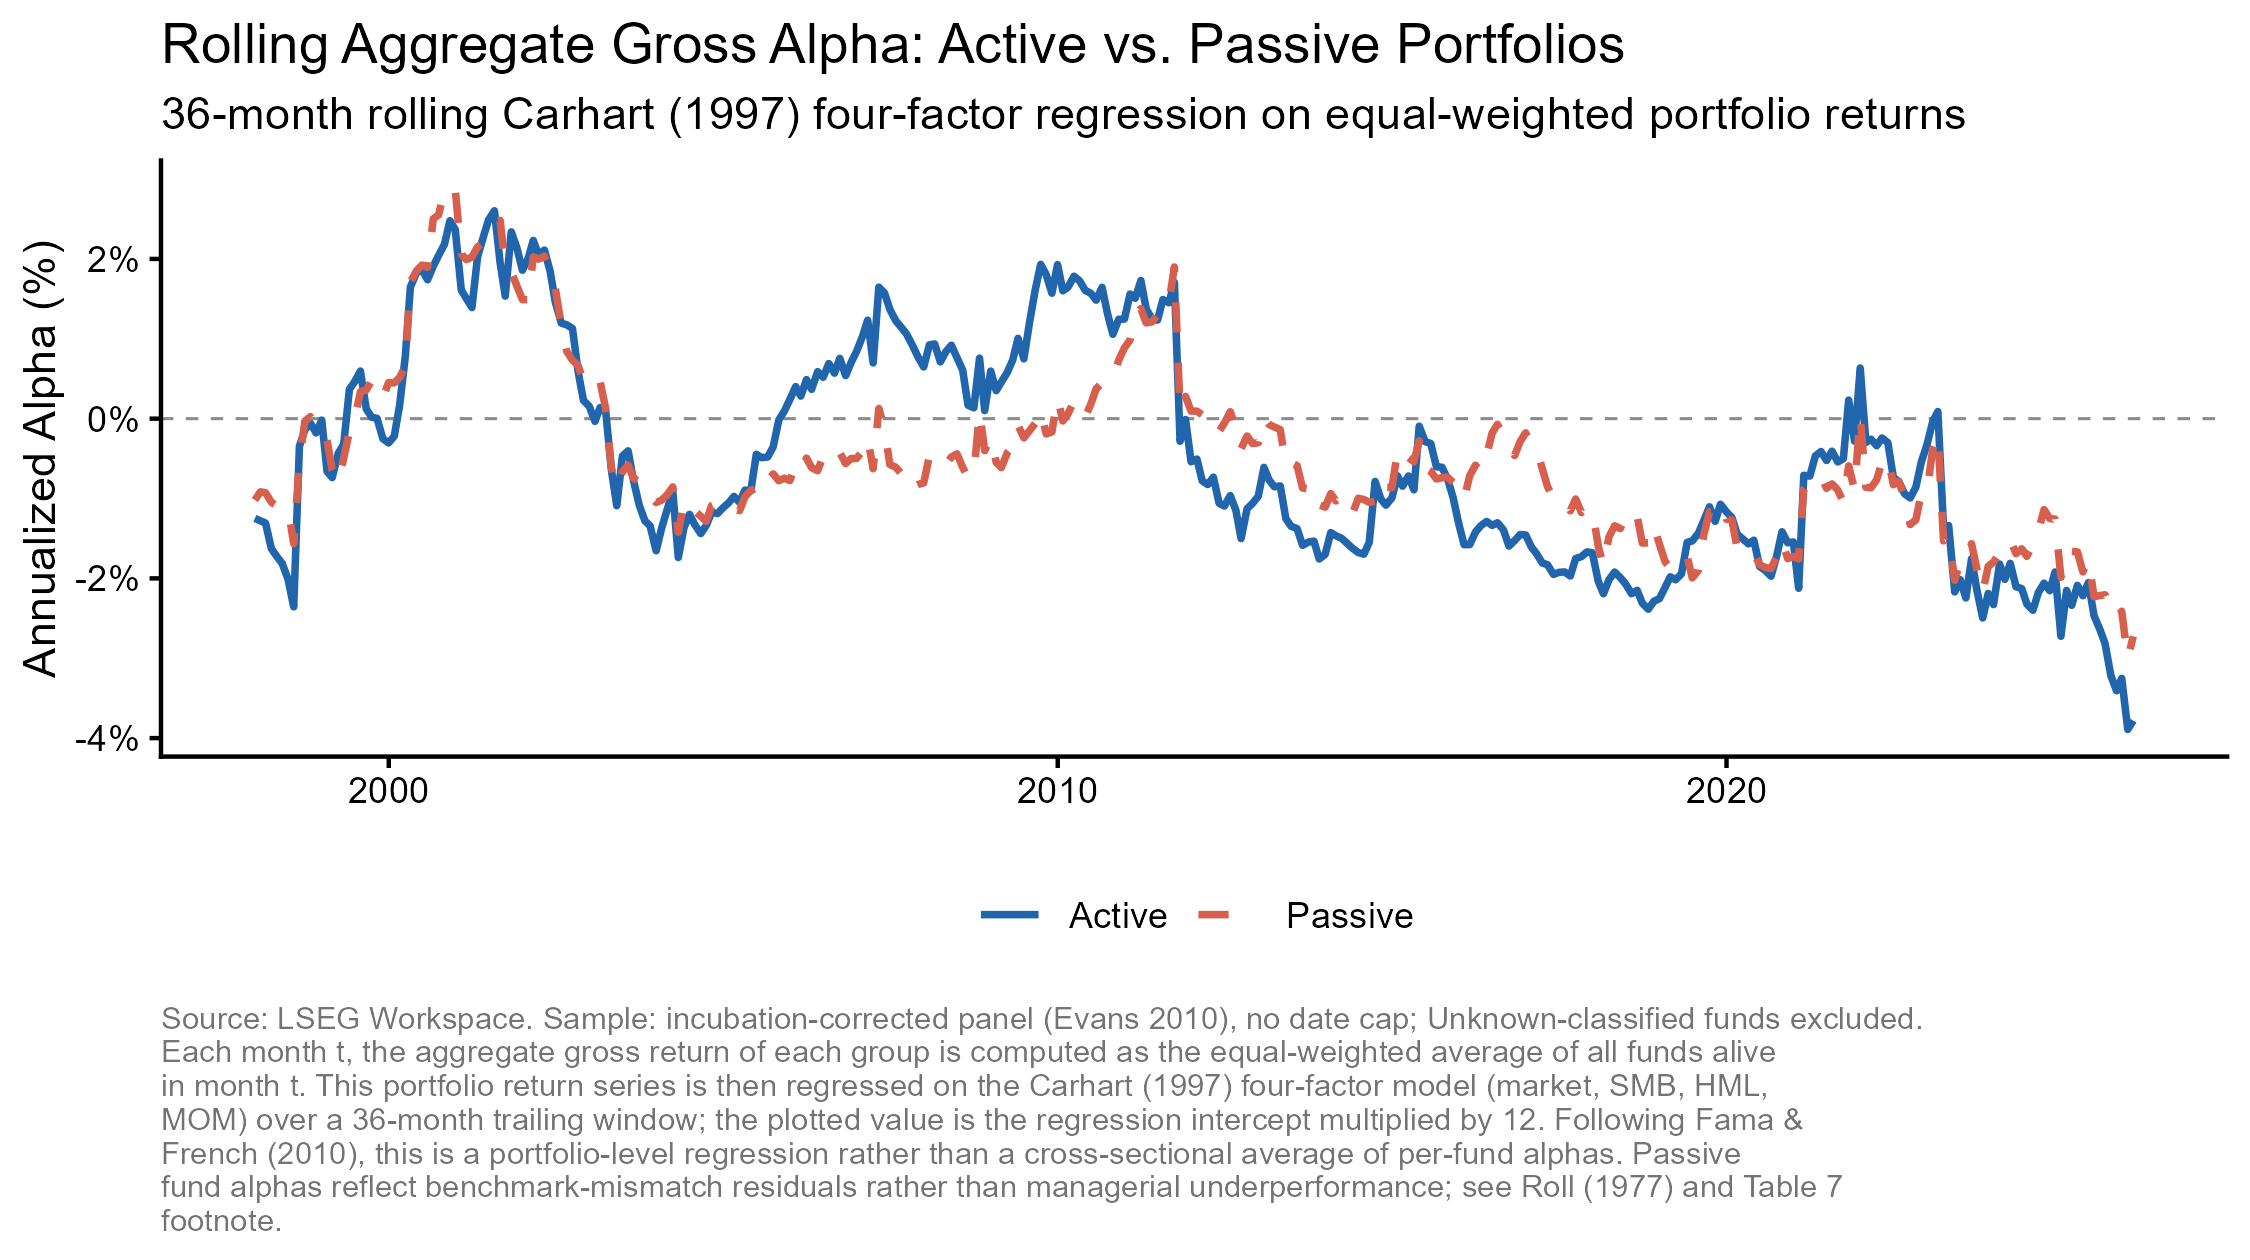
\includegraphics[width=\linewidth]{tables/fig_rolling_alphas}}{%
        \fbox{\parbox[c][4cm][c]{\linewidth}{\centering\footnotesize\texttt{fig\_rolling\_alphas.png}}}}
    \end{column}
    \begin{column}{0.42\textwidth}
      \begin{itemize}\itemsep5pt
        \item 36-month rolling Carhart gross alpha (EW).
        \item \textbf{Dot-com era}: alpha oscillates around zero.
        \item \textbf{2006–2011}: sustained positive alpha — the best era for active management.
        \item \textbf{Post-2011 collapse}: persistent and deepening negative alpha.
        \item Active and passive track closely — the gap is driven by fee drag.
      \end{itemize}
    \end{column}
  \end{columns}
\end{frame}

\begin{frame}{Factor Robustness}
  \begin{itemize}\itemsep5pt
    \item Main results estimated under Carhart (1997) four-factor model.
    \item \textbf{Appendix E} re-estimates under FF5 (Fama \& French 2015) and
          Carhart + Pastor–Stambaugh (2003) liquidity factor.
    \item Qualitative verdict \textbf{unchanged}: EW net alpha negative and significant;
          VW net alpha negative but of smaller magnitude.
    \item RMW and CMA absorb some dispersion but do not overturn the puzzle.
    \item Factor model choice \emph{does not} alter H1–H4 identification:
          behavioral channels are identified from flow--performance convexity,
          not from the level of alpha.
  \end{itemize}
\end{frame}

% ============================================================
%  PART IV — BOOTSTRAP & FDR
% ============================================================
\section{IV.\ Bootstrap \& FDR Decomposition}

\begin{frame}{Why Bootstrap? The Multiple-Testing Problem}
  \begin{itemize}\itemsep5pt
    \item With $N \approx 1{,}800$ funds, some will show extreme $t(\hat{\alpha})$
          \emph{by luck alone} — even if every fund's true alpha is zero.
    \item OLS $p$-values are fund-by-fund and ignore cross-sectional correlation.
    \item \textbf{Fama \& French (2010)} solution: joint calendar-month resampling
          preserves the cross-sectional correlation structure.
    \item Generate a ``zero-skill'' benchmark distribution for the \emph{cross-section}
          of $t$-statistics.
    \item \textbf{BSW (2010)} complement: use the marginal $p$-value distribution to
          decompose the cross-section into skilled / unskilled / zero-alpha funds.
  \end{itemize}
\end{frame}

\begin{frame}{FF (2010) Bootstrap: Design}
  \textbf{Steps}
  \begin{enumerate}\itemsep3pt
    \item Estimate $\hat{\alpha}_i$ for each fund; compute zero-alpha residuals
          $\tilde{r}_{i,t} = r_{i,t} - \hat{\alpha}_i$.
    \item Draw $B = 10{,}000$ bootstrap samples by resampling \emph{calendar months}
          (same months for all funds — preserves cross-section).
    \item Re-estimate Carhart on each bootstrapped series; record $t(\hat{\alpha}^b)$.
    \item Compare \emph{actual} cross-sectional $t$-percentiles to the simulated distribution.
  \end{enumerate}
  \vspace{6pt}
  \textbf{Key design choice}: simulated $t$-stats use \textbf{same Newey–West lag} as actual
  (apples-to-apples; was a confirmed bug in earlier versions, corrected in v2.5).
\end{frame}

\begin{frame}{Bootstrap Results \& FDR Decomposition}
  \begin{columns}[T]
    \begin{column}{0.45\textwidth}
      \textbf{Bootstrap: Left tail (losers)}
      \begin{itemize}\itemsep4pt
        \item Bottom 1\textsuperscript{st} percentile actual $t \approx -3.52$
              vs.\ simulated mean $\approx -2.37$.
        \item \alert{Left-tail rejection}: genuine underperformers exist.
      \end{itemize}
      \textbf{Bootstrap: Right tail (winners)}
      \begin{itemize}\itemsep4pt
        \item Top 99\textsuperscript{th} percentile actual $t \approx 2.43$
              vs.\ simulated mean $\approx 2.34$.
        \item Consistent with zero skill at the top.
      \end{itemize}
    \end{column}
    \begin{column}{0.52\textwidth}
      \textbf{BSW decomposition at $\gamma = 20\pct$}
      \vspace{4pt}\\
      \footnotesize
      \begin{tabular}{lrr}
        \toprule
        & Negative tail & Positive tail \\
        \midrule
        $\hat{\pi}_0$ (zero-alpha) & \multicolumn{2}{c}{$\mathbf{77.8\pct}$ ($N=1{,}815$)} \\
        Observed $S_\gamma$        & 28.9\% & 5.8\% \\
        False disc.\ $F_\gamma$    & \multicolumn{2}{c}{7.8\%} \\
        \textbf{True proportion}   & $\hat{\pi}^-_A = \mathbf{21.1\pct}$ & $\hat{\pi}^+_A = \mathbf{-2.0\pct}$ \\
        \bottomrule
      \end{tabular}
      \vspace{6pt}\\
      \small $\hat{\pi}^+_A < 0$: genuinely skilled mass does \emph{not exceed} the false-discovery
      rate. Storey estimator is conservative, so this is an upper-bound on skilled share.
    \end{column}
  \end{columns}
  \source{Barras, Scaillet \& Wermers (2010, JF)}
\end{frame}

\begin{frame}{Luck vs.\ Skill: CDF (Figure 3)}
  \begin{columns}[T]
    \begin{column}{0.55\textwidth}
      \IfFileExists{tables/fig_luck_vs_skill_combined.png}{%
        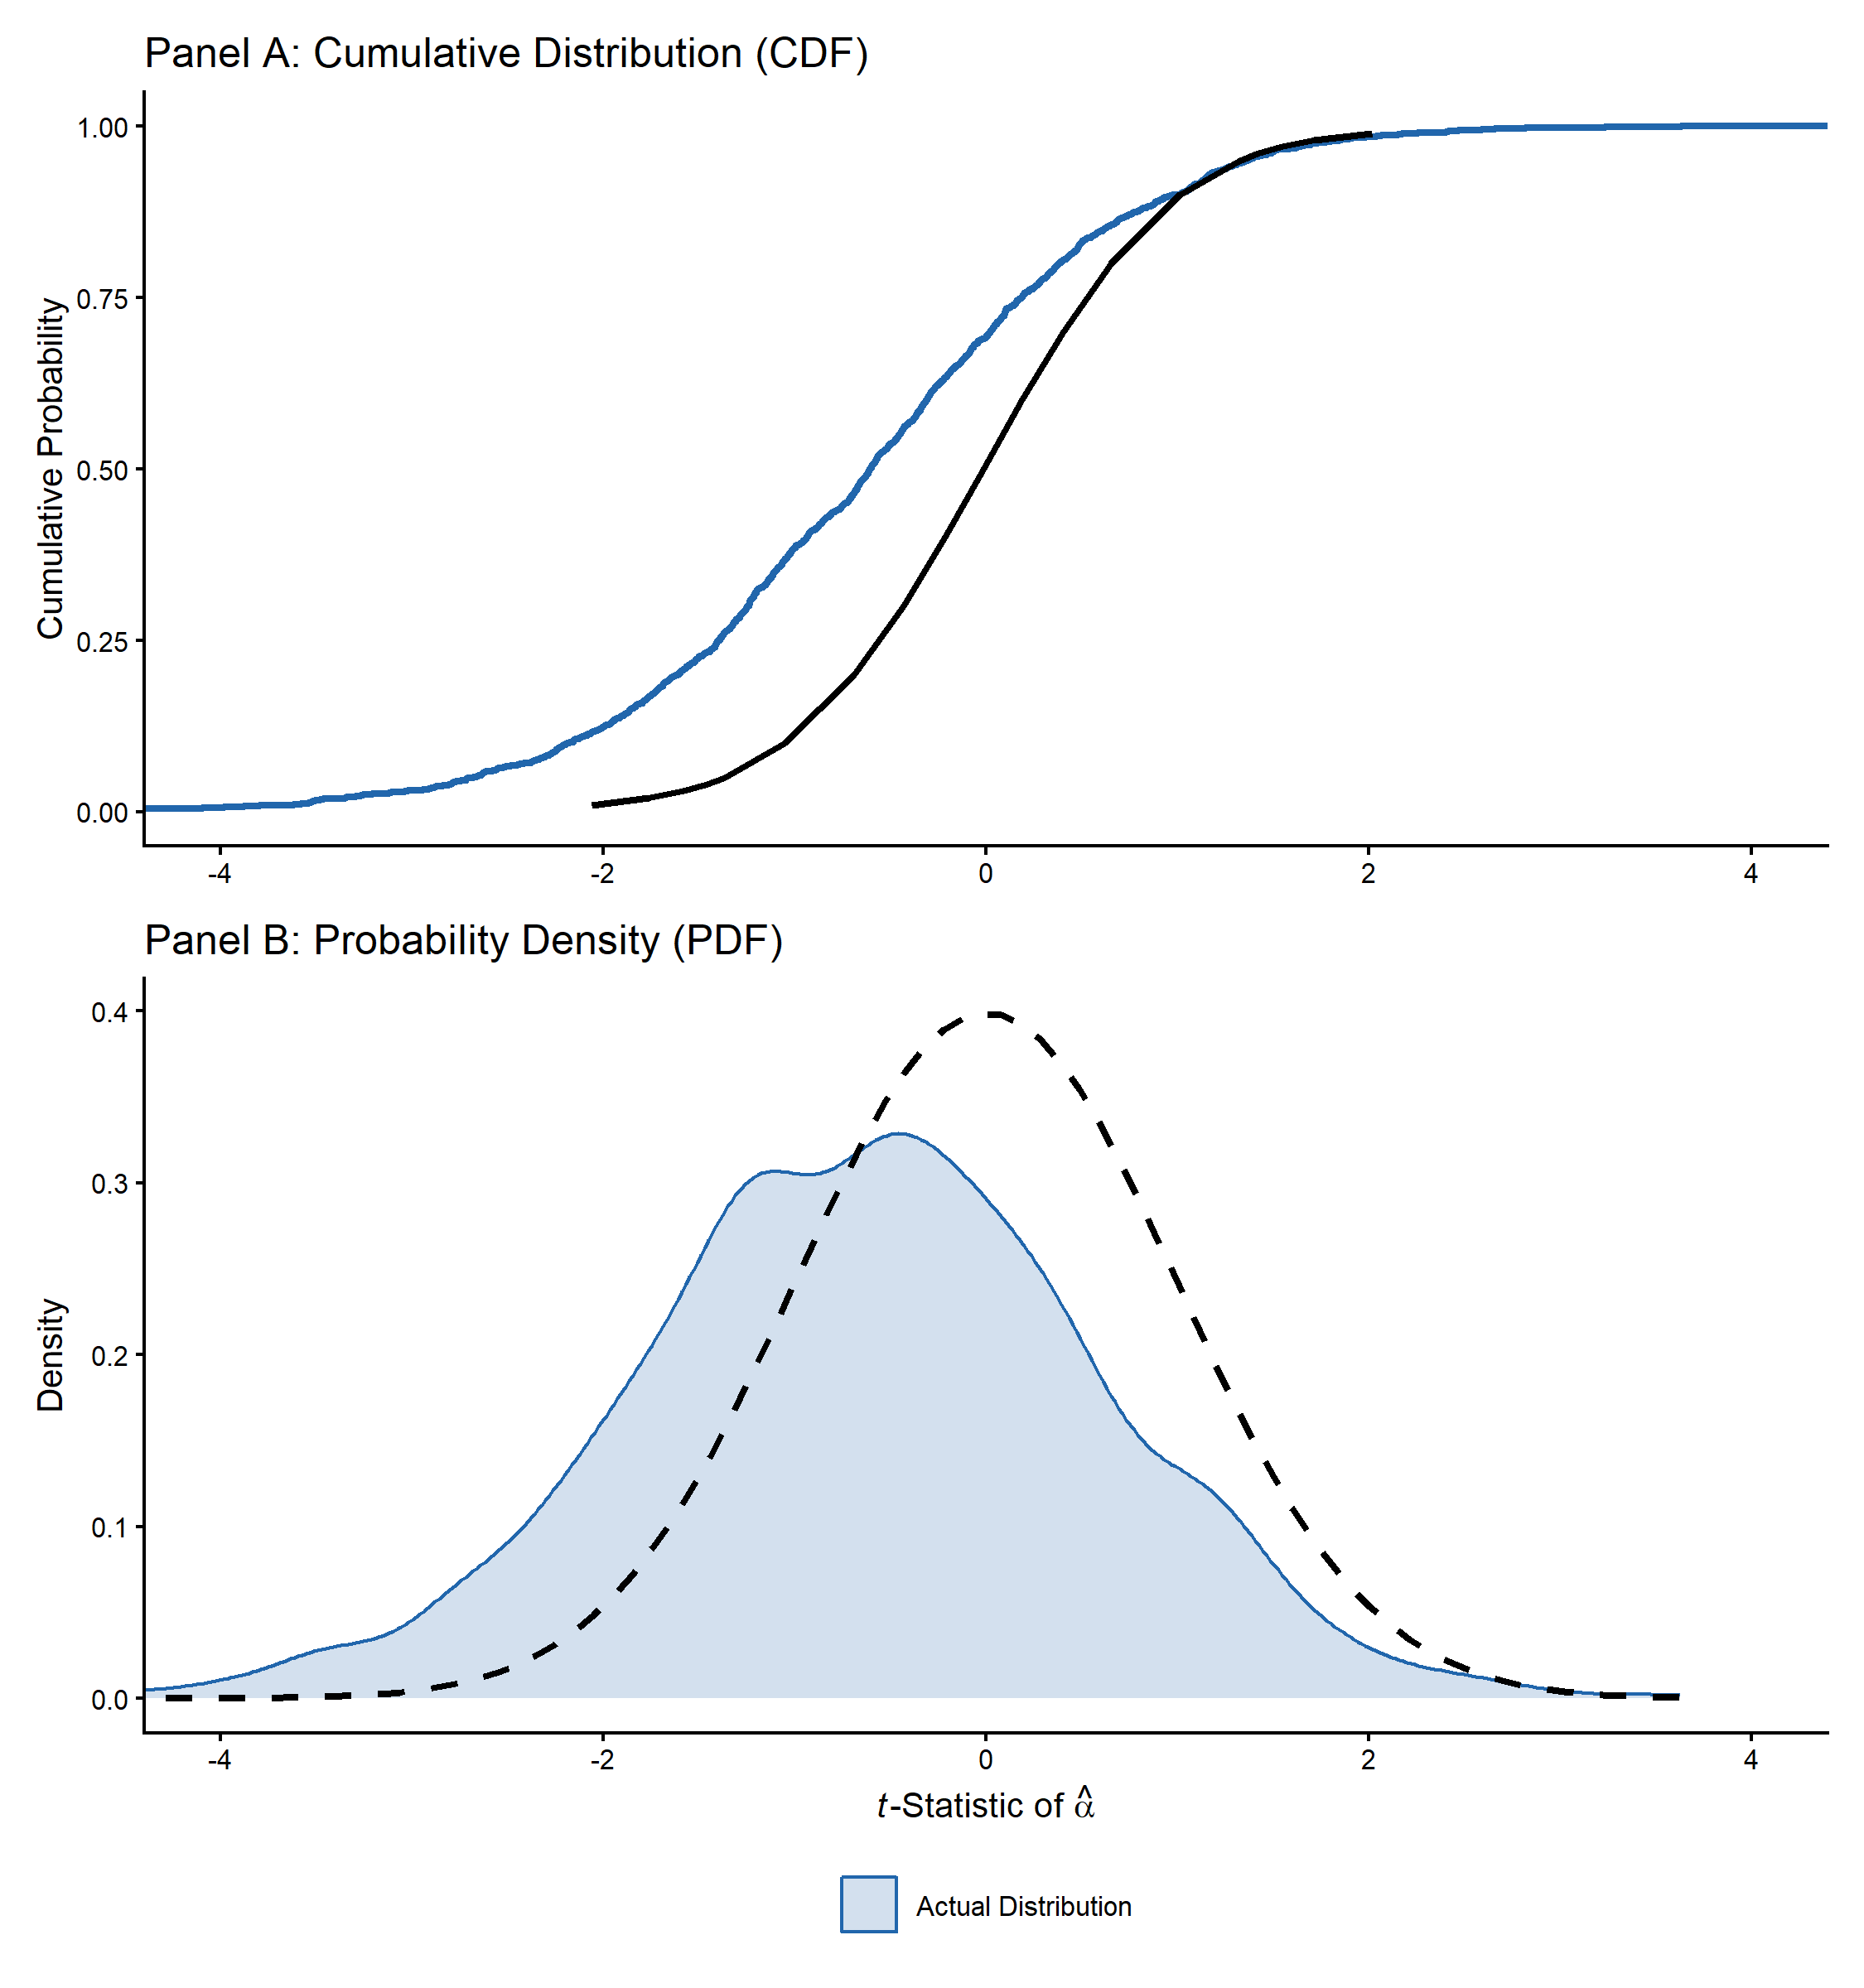
\includegraphics[width=\linewidth]{tables/fig_luck_vs_skill_combined}}{%
        \fbox{\parbox[c][4cm][c]{\linewidth}{\centering\footnotesize\texttt{fig\_luck\_vs\_skill\_combined.png}}}}
    \end{column}
    \begin{column}{0.42\textwidth}
      \begin{itemize}\itemsep5pt
        \item Actual CDF of $t(\hat{\alpha})$ \emph{shifted left} of the simulated
              zero-skill CDF.
        \item \textbf{Left tail}: actual lies far below simulated — genuine underperformers.
        \item \textbf{Right tail}: actual tracks simulated — no evidence of genuine skill.
        \item Interpretation: the active fund industry produces a fat left tail,
              not a fat right tail.
      \end{itemize}
    \end{column}
  \end{columns}
\end{frame}

% ============================================================
%  PART V — STRUCTURAL BREAK & SUB-PERIODS
% ============================================================
\section{V.\ Structural Break \& Sub-Period Analysis}

\begin{frame}{Bai–Perron Test: Setup \& BIC Solution}
  \begin{itemize}\itemsep5pt
    \item Applied to the 12-month trailing mean of the monthly cross-sectional EW
          rolling Carhart gross alpha series.
    \item \textbf{Bai \& Perron (1998, 2003)}: BIC-optimal number of breaks selected;
          confidence intervals via Newey–West HAC (Andrews 1991).
    \item BIC selects \textbf{5 breaks}, defining 6 regimes.
    \item Minimum segment length: 36 months (BSW reliability constraint).
    \item \textbf{Adopted partition}: 3 regimes — Breaks 1–3 pooled into P1,
          Break 5 pooled into P3 (sub-60-month segments not reliable for FF/BSW inference).
  \end{itemize}
\end{frame}

\begin{frame}{Structural Break Figure (Figure D.1)}
  \begin{columns}[T]
    \begin{column}{0.60\textwidth}
      \IfFileExists{tables/fig_breaktest.png}{%
        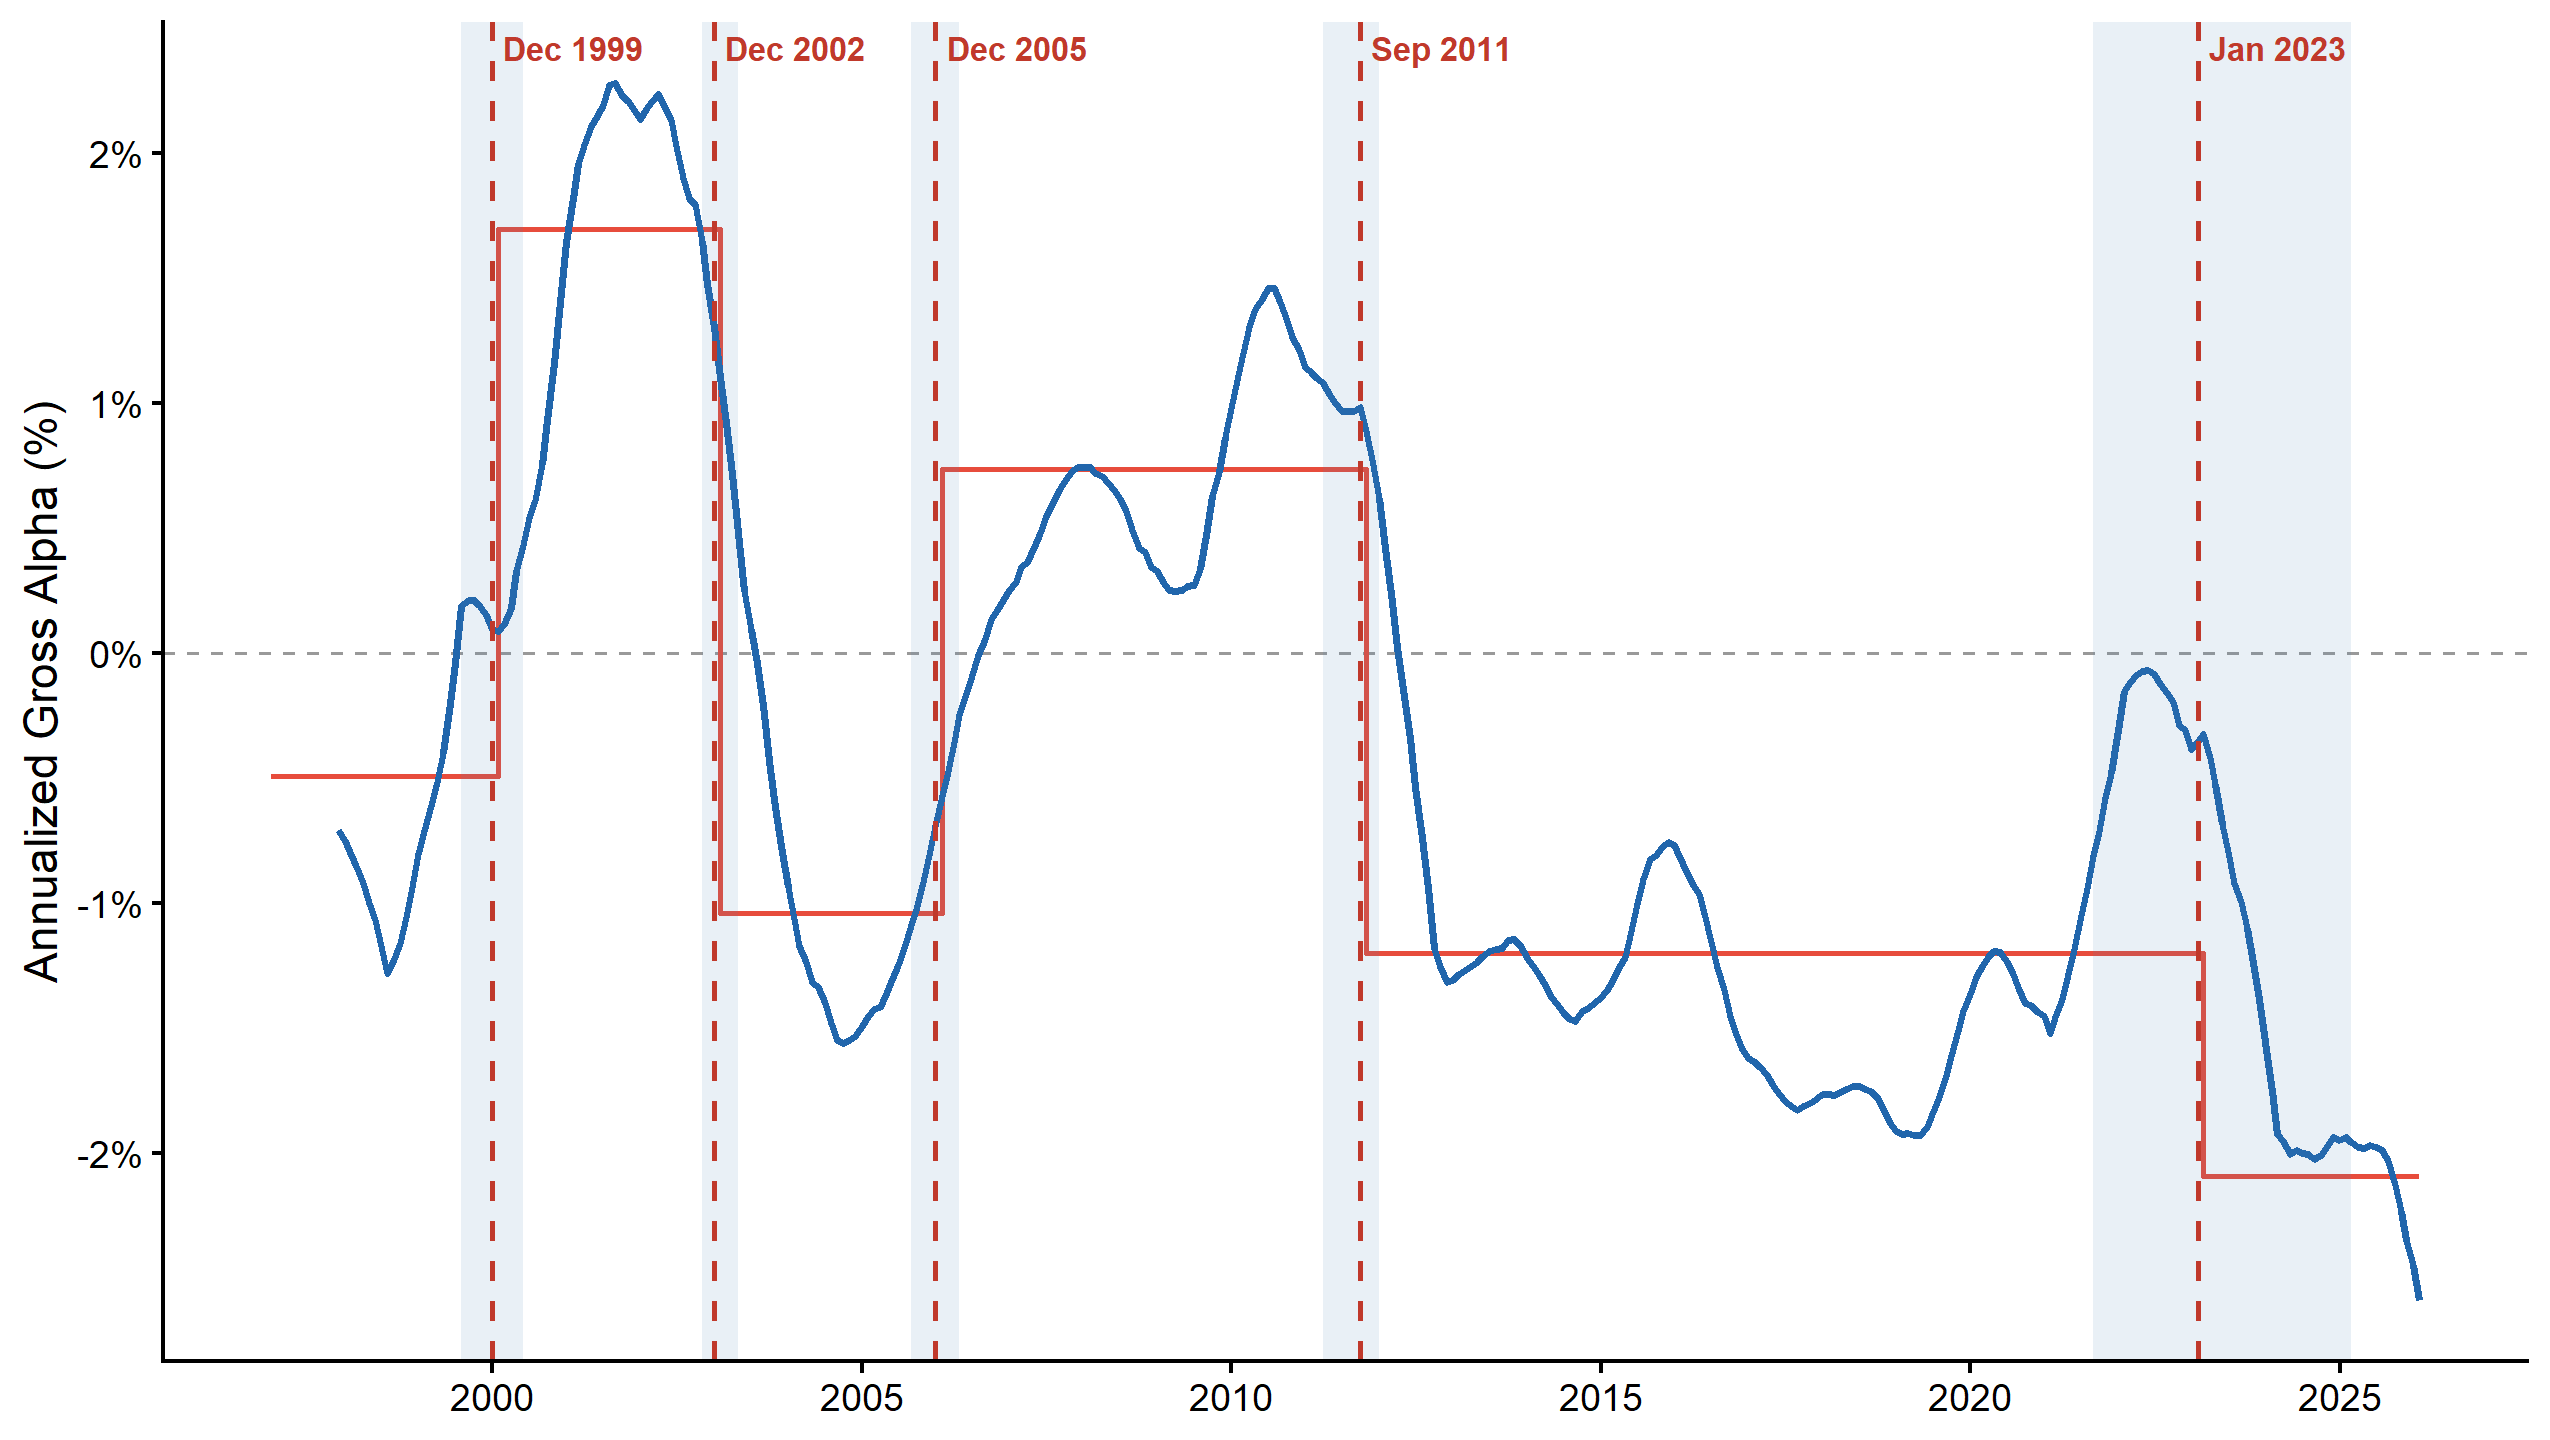
\includegraphics[width=\linewidth]{tables/fig_breaktest}}{%
        \fbox{\parbox[c][4cm][c]{\linewidth}{\centering\footnotesize\texttt{fig\_breaktest.png}}}}
    \end{column}
    \begin{column}{0.38\textwidth}
      \footnotesize
      \begin{tabular}{lcc}
        \toprule
        Break & Date & 95\% CI \\
        \midrule
        1 & Dec 1999 & wide \\
        2 & Dec 2002 & wide \\
        3 & Dec 2005 & 8 months \\
        \textbf{4} & \textbf{Nov 2011} & \textbf{9 months} \\
        5 & Jan 2023 & 31 months \\
        \bottomrule
      \end{tabular}
      \vspace{6pt}\\
      \textbf{Break 4} is the key structural event:\\
      $+0.74\pct \to -1.20\pct$ (\textbf{194 bp shift}).\\
      Tightest CI in the sample.\\
      Not previously reported with this methodology.
    \end{column}
  \end{columns}
\end{frame}

\begin{frame}{Sub-Period Performance \& Skill Decomposition}
  \footnotesize
  \begin{tabular}{lrrrrr}
    \toprule
    & \multicolumn{2}{c}{Active net $\alpha$ (\%, ann.)} & $\hat{\pi}_0$ & $\hat{\pi}^-_A$ & $\hat{\pi}^+_A$ \\
    \cmidrule(l){2-3}
    Period & EW & VW & & at $\gamma=20\pct$ & at $\gamma=20\pct$ \\
    \midrule
    P1: Jan 1995–Dec 2005 & $-1.34^{*}$ & $-0.93$ & 81.4\% & 10.8\% & $+3.3\%$ \\
    P2: Jan 2006–Sep 2011 & $-0.67$    & $-0.85$ & 87.3\% & $3.1\%$ & $+8.4\%$ \\
    P3: Oct 2011–Feb 2026 & $-2.50^{***}$& $-1.41^{***}$ & 60.8\% & 35.4\% & $-3.7\%$ \\
    \midrule
    Full period           & $-1.36^{***}$& $-0.90^{**}$  & 77.8\% & 21.1\% & $-2.0\%$ \\
    \bottomrule
  \end{tabular}
  \vspace{6pt}
  \begin{itemize}\itemsep4pt
    \item \textbf{P2} is the ``golden era'' — positive gross alpha, positive skilled share ($8.4\pct$).
    \item \textbf{P3 collapse}: $\hat{\pi}^-_A$ jumps to 35.4\%; skilled share goes negative.
    \item The regime change is not a mean-shift — it \emph{reshapes the cross-sectional skill distribution}.
    \item \textbf{Three interpretations} of P3 collapse discussed in Section 6.3 (skill erosion /
          factor proliferation / behavioral crowding).
  \end{itemize}
\end{frame}

% ============================================================
%  PART VI — ACTIVENESS & PERSISTENCE
% ============================================================
\section{VI.\ Activeness \& Persistence}

\begin{frame}{Activeness Measures \& Quintile Sorts}
  \begin{columns}[T]
    \begin{column}{0.50\textwidth}
      \textbf{Two measures}
      \begin{itemize}\itemsep4pt
        \item $1 - R^2$: residual from 36-month rolling Carhart regression
              (Amihud \& Goyenko 2013). Higher = more active.
        \item \textbf{Tracking Error}: annualised SD of monthly return minus
              benchmark return (Cremers \& Petajisto 2009).
      \end{itemize}
      \vspace{6pt}
      \textbf{Sort design}
      \begin{itemize}\itemsep4pt
        \item Funds sorted into quintiles Q1–Q5 annually.
        \item Q1: closet indexers ($1-R^2 \approx 0.032$).
        \item Q5: most active ($1-R^2 \approx 0.211$; ER = 1.36\%).
      \end{itemize}
    \end{column}
    \begin{column}{0.46\textwidth}
      \footnotesize
      \begin{tabular}{lrrrr}
        \toprule
        & Act. & TNA & ER & Car.\ $\alpha$ \\
        & $1-R^2$ & \$M & \% & EW gross \\
        \midrule
        Q1 (Closet) & 0.032 & 3,420 & 0.80 & $-0.60^{*}$ \\
        Q2          & 0.057 & 4,615 & 0.95 & $-0.34$ \\
        Q3          & 0.076 & 2,489 & 1.04 & $-0.32$ \\
        Q4          & 0.100 & 1,425 & 1.10 & $-0.22$ \\
        Q5 (Active) & 0.211 &   980 & 1.36 & $+0.10$ \\
        \midrule
        Q5$-$Q1     &       &       &      & $+0.69^{*}$ \\
        \bottomrule
      \end{tabular}
      \vspace{4pt}\\
      \tiny EW gross alpha; Carhart four-factor; NW $t$-stats.
    \end{column}
  \end{columns}
\end{frame}

\begin{frame}{Activeness: Interpretation}
  \begin{itemize}\itemsep6pt
    \item \textbf{Gross} alpha is positive for Q5 and the Q5–Q1 spread is marginally significant.
    \item But Q5 carries the \emph{highest fees} (ER = 1.36\%): \textbf{net alpha is negative}.
    \item Result aligns with \textbf{Outcome 1} from the activeness methodology:
          most-active funds underperform most severely \emph{net of fees}.
    \item \textbf{Closet indexers} (Q1) collect near-market returns but charge active-style fees
          — the worst of both worlds for investors.
    \item Q5 funds are disproportionately small (TNA \$980M vs.\ Q1 \$3,420M) —
          consistent with Berk–Green decreasing returns to scale.
    \item Forward link to \textbf{H3}: high-activeness funds also have extreme MAX12
          (lottery appeal), which partly explains why flows persist despite negative net alpha.
  \end{itemize}
\end{frame}

\begin{frame}{Performance Persistence}
  \begin{columns}[T]
    \begin{column}{0.52\textwidth}
      \textbf{KTWW (2006) bootstrap on decile cohorts}
      \begin{itemize}\itemsep4pt
        \item Formation period: rank funds by past $t(\hat{\alpha})$ into deciles.
        \item Holding period: compute next-period EW decile alpha.
        \item Bootstrap: resample to test if holding-period $t(\hat{\alpha})$ is
              significant relative to zero-skill null.
      \end{itemize}
      \vspace{4pt}
      \textbf{Key results}
      \begin{itemize}\itemsep4pt
        \item \alert{Left tail (D1): significant loser persistence confirmed.}
        \item \textbf{Right tail (D10): no significant winner persistence.}
        \item Pattern is strongest in P3; consistent with BSW collapse in $\hat{\pi}^+_A$.
        \item Cross-regime design confirms structural heterogeneity.
      \end{itemize}
    \end{column}
    \begin{column}{0.45\textwidth}
      \begin{block}{Interpretation}
        Loser persistence \emph{without} winner persistence is the asymmetric footprint
        of the behavioral mechanisms tested in H1–H4:
        \begin{itemize}\itemsep4pt
          \item Winners get chased (flows erode alpha — BG).
          \item Losers get \emph{held} (flows fail to exit — behavioral).
        \end{itemize}
      \end{block}
    \end{column}
  \end{columns}
\end{frame}

% ============================================================
%  PART VII — BEHAVIORAL FRAMEWORK
% ============================================================
\section{VII.\ Behavioral Framework}

\begin{frame}{The Residual Puzzle}
  \begin{columns}[T]
    \begin{column}{0.48\textwidth}
      \textbf{What BG (2004) explains}
      \begin{itemize}\itemsep4pt
        \item VW net alpha $\approx -0.90\pct$ (close to zero, fees paid out).
        \item Capital-weighted investors collectively break even before fees.
        \item Flows chase skilled managers; competition drives equilibrium.
      \end{itemize}
    \end{column}
    \begin{column}{0.48\textwidth}
      \textbf{What BG leaves unexplained}
      \begin{itemize}\itemsep4pt
        \item \alert{EW–VW gap of $\approx 46\bp$}: small funds underperform disproportionately.
        \item Loser persistence: underperformers retain capital.
        \item State-dependence: flows change \emph{character} across sentiment regimes.
        \item Lottery-like flows unrelated to risk-adjusted expected returns.
      \end{itemize}
    \end{column}
  \end{columns}
  \vspace{8pt}
  \begin{block}{Behavioral Claim}
    The cross-sectional heterogeneity and the loser-flow anomaly require
    at least one behavioral channel beyond rational capital allocation.
  \end{block}
\end{frame}

\begin{frame}{Common Regression Architecture}
  \textbf{Sirri–Tufano (1998) piecewise flow–performance specification, augmented:}
  \vspace{4pt}
  \[
    \text{Flow}_{i,t+1} = \beta_1 R^{\text{LOW}}_{i,t} + \beta_2 R^{\text{MID}}_{i,t}
    + \beta_3 R^{\text{HIGH}}_{i,t}
    + \delta_1 R^{\text{LOW}}_{i,t} \cdot Z_t
    + \delta_2 R^{\text{MID}}_{i,t} \cdot Z_t
    + \delta_3 R^{\text{HIGH}}_{i,t} \cdot Z_t
    + \gamma \mathbf{X}_{i,t} + \mu_i + \varepsilon_{i,t}
  \]
  \vspace{2pt}
  \begin{columns}[T]
    \begin{column}{0.45\textwidth}
      \textbf{Rank segments}\\[3pt]
      \footnotesize
      \begin{tabular}{lll}
        $R^{\text{LOW}}$  & $\min(\text{rank},0.20)$           & Bottom quintile \\
        $R^{\text{MID}}$  & middle 60\%                        & \\
        $R^{\text{HIGH}}$ & $\max(\text{rank}-0.80,0)$         & Top quintile \\
      \end{tabular}
    \end{column}
    \begin{column}{0.52\textwidth}
      \textbf{State variables $Z_t$}\\[3pt]
      \footnotesize
      \begin{tabular}{ll}
        $D^{\text{SENT}}$ & Baker–Wurgler sentiment (binary) \\
        $\text{SENT}^\perp$ & BW orthogonalized to macro \\
        $D^{\text{AAII}}$ & AAII Bull–Bear spread (binary) \\
        $D^{\text{MD}}$   & Margin debt growth (H2 only) \\
        $D^{\text{INV-PCR}}$ & Inverse put/call ratio (H2 only) \\
      \end{tabular}
    \end{column}
  \end{columns}
  \vspace{6pt}
  \footnotesize Fund FE for H1–H3; Lipper $\times$ yearmo FE for H4.
  Two-way clustering on Ticker and calendar month (Petersen 2009).
  December observations dropped (year-end distribution contamination).
\end{frame}

% ============================================================
%  PART VIII — H1
% ============================================================
\section{VIII.\ H1: Sentiment-Convexity}

\begin{frame}{H1: Hypothesis \& Prediction}
  \begin{block}{H1: Sentiment-Convexity}
    During high-sentiment regimes, the winner-segment flow response steepens
    ($\delta_3 > 0$), amplifying flow–performance convexity.
  \end{block}
  \vspace{8pt}
  \begin{columns}[T]
    \begin{column}{0.48\textwidth}
      \textbf{Behavioral mechanism}
      \begin{itemize}\itemsep4pt
        \item Representativeness heuristic (Kahneman \& Tversky 1974): investors
              extrapolate recent winner returns as evidence of skill.
        \item Sentiment amplifies this extrapolation.
        \item Prediction: $\delta_3 > 0$ (convexity amplified at the top).
        \item Secondary: $\delta_3 - \delta_1 > 0$ (asymmetry widens).
      \end{itemize}
    \end{column}
    \begin{column}{0.48\textwidth}
      \textbf{Rational null}
      \begin{itemize}\itemsep4pt
        \item BG: sentiment should not alter the flow–performance mapping.
        \item Search-cost story (ST 1998): marketing, not sentiment.
        \item Prediction: $\delta_1 = \delta_2 = \delta_3 = 0$.
      \end{itemize}
    \end{column}
  \end{columns}
\end{frame}

\begin{frame}{H1: Results}
  \footnotesize
  \begin{tabular}{llllr}
    \toprule
    State proxy & Joint $\chi^2$ (df=3) & Headline $z$ & 1-sided $p$ & Decision \\
    \midrule
    $D^{\text{SENT}}$ & 9.13 ($p=0.028$) & $+0.06$ & $0.475$ & \yes\ (asymmetry +) \\
    $\text{SENT}^\perp$ & 6.92 ($p=0.074$) & $-0.36$ & $0.639$ & \yes\ (asymmetry $-$) \\
    $D^{\text{AAII}}$ & \textbf{11.02 ($p=0.012$)} & $\mathbf{+2.11}$ & $\mathbf{0.018}$ & \textbf{\yes\ (asymmetry +)} \\
    \bottomrule
  \end{tabular}
  \vspace{8pt}
  \begin{itemize}\itemsep4pt
    \item Joint $\chi^2$ rejects the null that all three interaction terms are zero in all specs.
    \item AAII spec: both joint test and asymmetry $z$ significant.
    \item BW SENT directions mixed — robustness with AAII is the cleaner signal.
    \item Lagged-spec robustness: qualitatively consistent.
    \item \textbf{Interpretation}: flow convexity is state-dependent; high-sentiment periods
          disproportionately amplify winner-chasing — consistent with
          \textbf{representativeness heuristic}, not rational search-cost adjustment.
  \end{itemize}
\end{frame}

% ============================================================
%  PART IX — H2
% ============================================================
\section{IX.\ H2: Disposition Effect / Illusion of Control}

\begin{frame}{H2: Hypothesis \& Discrimination Design}
  \begin{block}{H2: Disposition Effect / Illusion of Control}
    High financial stress flattens the loser-segment outflow response —
    investors fail to exit underperformers when they are most constrained.
  \end{block}
  \vspace{8pt}
  \textbf{Two competing behavioral mechanisms for loser stickiness:}
  \vspace{4pt}
  \begin{columns}[T]
    \begin{column}{0.48\textwidth}
      \textbf{Disposition Effect (Shefrin \& Statman 1985)}
      \begin{itemize}\itemsep4pt
        \item Loss aversion prevents realising losses.
        \item Predicts: $\delta_1 < 0$ (loser exit \emph{further} attenuated).
        \item Proxy: Inverse Put/Call Ratio ($D^{\text{INV-PCR}}$).
      \end{itemize}
    \end{column}
    \begin{column}{0.48\textwidth}
      \textbf{Brunnermeier–Pedersen (2009) Margin Call}
      \begin{itemize}\itemsep4pt
        \item Margin pressure forces liquidation of \emph{liquid} assets;
              illiquid fund positions retained.
        \item Predicts: $\delta_1 > 0$ (loser slope \emph{steepens} under margin stress).
        \item Proxy: Margin Debt growth ($D^{\text{MD}}$).
      \end{itemize}
    \end{column}
  \end{columns}
\end{frame}

\begin{frame}{H2: Results}
  \footnotesize
  \begin{tabular}{llllr}
    \toprule
    State proxy & Joint $\chi^2$ (df=3) & $\delta_1$ $z$ & 1-sided LEFT $p$ & Decision \\
    \midrule
    $D^{\text{MD,Det}}$ & \textbf{11.24 ($p=0.010$)} & $+2.15$ & $0.984$ &
      \yes\ \textbf{(BP margin-call)} \\
    $D^{\text{INV-PCR}}$ & 0.44 ($p=0.931$) & $-0.20$ & $0.420$ &
      \no\ (disposition) \\
    Discriminant & 7.52 ($p=0.057$) & $+1.91$ & $0.972$ &
      \yes\ (BP direction) \\
    \bottomrule
  \end{tabular}
  \vspace{8pt}
  \begin{itemize}\itemsep4pt
    \item \textbf{$\delta_1 > 0$} paired with \textbf{high one-sided $p$}: rejects the
          disposition prediction ($\delta_1 < 0$) decisively.
    \item High margin debt \emph{steepens} the loser segment — losers bleed \emph{more}
          under margin stress, not less.
    \item This is the \textbf{Brunnermeier–Pedersen (2009)} liquidity spiral signature:
          investors forced to sell losers for \emph{liquidity}, not holding them out of loss-aversion.
    \item INV-PCR spec: clean null — disposition effect not operative in this sample.
    \item \textbf{Implication}: loser stickiness is a \emph{margin-call / liquidity effect},
          not classical disposition.
  \end{itemize}
\end{frame}

% ============================================================
%  PART X — H3
% ============================================================
\section{X.\ H3: Lottery Demand}

\begin{frame}{H3: Hypothesis \& Proxies}
  \begin{block}{H3: Lottery Demand and Skewness Preference}
    Investors with gambling preferences allocate to funds with extreme recent
    upside potential, weakening exit discipline among underperformers with
    lottery-like return profiles.
  \end{block}
  \vspace{8pt}
  \textbf{Three lottery proxies tested:}
  \vspace{4pt}
  \begin{columns}[T]
    \begin{column}{0.32\textwidth}
      \textbf{ActR2}\\
      $1 - R^2$ activeness\\
      (Amihud–Goyenko 2013)\\
      \small Proxy for benchmark deviation
    \end{column}
    \begin{column}{0.32\textwidth}
      \textbf{ActSkew}\\
      Idiosyncratic skewness\\
      of fund returns\\
      \small Proxy for return asymmetry
    \end{column}
    \begin{column}{0.32\textwidth}
      \textbf{MAX12}\\
      Maximum monthly return\\
      in prior 12 months\\
      \small BFL (2011) lottery proxy
    \end{column}
  \end{columns}
  \vspace{8pt}
  \footnotesize
  Barberis \& Huang (2008): CPT investors overprice positively skewed assets.
  Kumar (2009): retail investors demand lottery stocks.
  Cheng et al.\ (2025): MAX weakens loser exit in mutual funds.
\end{frame}

\begin{frame}{H3: Results}
  \footnotesize
  \begin{tabular}{lllr}
    \toprule
    Proxy & Joint $\chi^2$ (df=2) & Headline $z$ (1-sided $p$) & Decision \\
    \midrule
    ActR2   & 2.25 ($p=0.325$)          & $-0.02$ ($p=0.506$) & \no \\
    ActSkew & 1.95 ($p=0.378$)          & $+0.25$ ($p=0.400$) & \no \\
    \textbf{MAX12}   & \textbf{11.33 ($p=0.003$)} & $+1.54$ ($p=0.062$) & \textbf{\yes} \\
    \bottomrule
  \end{tabular}
  \vspace{8pt}
  \begin{itemize}\itemsep4pt
    \item Only \textbf{MAX12} clears the statistical threshold.
    \item ActR2 null: in earlier run on \texttt{panel\_trimmed} there was a spurious
          ``anti-premium'' result ($p=0.990$); \texttt{panel\_incubation} delivers a clean null.
    \item \textbf{Behavioral mechanism}: investors chase funds with \emph{recent extreme maximum returns},
          not funds that deviate from benchmark in the abstract.
    \item ``Delegated lottery'' interpretation: retail investors outsource gambling
          to active managers with the best recent headline number.
    \item Non-monotone, Q5-concentrated effect: survives Patton–Timmermann (2010)
          monotonicity test.
  \end{itemize}
\end{frame}

% ============================================================
%  PART XI — H4
% ============================================================
\section{XI.\ H4: Fee Elasticity}

\begin{frame}{H4: Hypothesis \& Results}
  \begin{block}{H4: Fee Elasticity}
    During high-sentiment regimes, investors become less sensitive to expense ratios
    — the negative flow–fee relationship is attenuated ($\psi > 0$).
  \end{block}
  \vspace{6pt}
  \footnotesize
  \begin{tabular}{lllr}
    \toprule
    State proxy & Joint $\chi^2$ (df=4) & Headline $z$ (1-sided $p$) & Decision \\
    \midrule
    $D^{\text{SENT}}$   & 4.45 ($p=0.349$) & $+0.74$ ($p=0.231$) & \no \\
    $\text{SENT}^\perp$ & 4.46 ($p=0.347$) & $+0.01$ ($p=0.496$) & \no \\
    $D^{\text{AAII}}$   & 5.17 ($p=0.270$) & $+1.36$ ($p=0.087$) & \no \\
    \bottomrule
  \end{tabular}
  \vspace{8pt}
  \begin{columns}[T]
    \begin{column}{0.48\textwidth}
      \textbf{H4 fails to reject}
      \begin{itemize}\itemsep4pt
        \item No sentiment proxy generates a significant fee-elasticity amplification.
        \item Consistent with the \textbf{rational null}: investors process fees
              regardless of market sentiment.
      \end{itemize}
    \end{column}
    \begin{column}{0.48\textwidth}
      \textbf{Policy implication}
      \begin{itemize}\itemsep4pt
        \item Regulatory focus on fee disclosure is \emph{partly justified}.
        \item Behavioral distortions in this sample operate through
              flow–performance \emph{convexity}, not fee processing.
        \item Disclosure reform alone will not fix the cross-sectional puzzle.
      \end{itemize}
    \end{column}
  \end{columns}
\end{frame}

% ============================================================
%  PART XII — PPF
% ============================================================
\section{XII.\ Psychological Premium Framework}

\begin{frame}{Shadow Price: Theory}
  \textbf{Motivation}: convert behavioral flow evidence into welfare-relevant units.
  \vspace{6pt}
  \textbf{Flow indifference condition} $d\,\text{Flow} = 0$:
  \[
    \text{SP}_t \;=\; \frac{dR}{d\,\text{AS}}\bigg|_{d\text{Flow}=0}
    \;=\; -\frac{\eta + \phi \cdot D^{\text{HIGH}}_t}
                {\beta_q + \delta_q \cdot D^{\text{HIGH}}_t}
  \]
  \begin{itemize}\itemsep5pt
    \item $\text{SP}_t$: rank points of performance the marginal investor sacrifices
          per unit of lottery exposure.
    \item Estimated separately for low-sentiment ($D^{\text{SENT}}=0$) and
          high-sentiment ($D^{\text{SENT}}=1$) regimes.
    \item Converted to \textbf{alpha basis points} via momentum-quintile rank-to-alpha
          mapping ($Q5-Q1 = 2.150\pct$ p.a.\ $\Rightarrow$ 269 bp/rank-point).
  \end{itemize}
\end{frame}

\begin{frame}{Shadow Price: Results}
  \footnotesize
  \begin{tabular}{llrrrr}
    \toprule
    Lottery & Seg. & $\text{SP}_{\text{low}}$ [SE] & $\text{SP}_{\text{high}}$ [SE] & Diff [SE] & $p$ \\
    \midrule
    ActR2   & $R^{\text{MID}}$ & 0.036 [0.030] & 0.059 [0.047] & 0.023 [0.045] & 0.694 \\
    ActSkew & $R^{\text{MID}}$ & $-$0.029 [0.029] & $-$0.056 [0.057] & $-$0.027 [0.061] & 0.328 \\
    \textbf{MAX12} & $R^{\text{MID}}$ & $-$\textbf{0.049} [0.031] & $-$\textbf{0.219} [0.072] &
    $-$\textbf{0.170} [0.076] & $\mathbf{0.013^{**}}$ \\
    MAX12   & $R^{\text{LOW}}$ & $-$0.022 [0.014] & $-$0.101 [0.050] & $-$0.079 [0.050] & $0.056^{*}$ \\
    MAX12   & $R^{\text{HIGH}}$& $-$0.009 [0.006] & $-$0.030 [0.010] & $-$0.021 [0.011] & $0.030^{*}$ \\
    \bottomrule
  \end{tabular}
  \vspace{8pt}
  \begin{columns}[T]
    \begin{column}{0.48\textwidth}
      \textbf{Basis-point translation (MAX12, $R^{\text{MID}}$)}
      \begin{itemize}\itemsep3pt
        \item Low sentiment: $|0.049| \times 269 \approx \mathbf{13\bp}$ per SD.
        \item High sentiment: $|0.219| \times 269 \approx \mathbf{59\bp}$ per SD.
        \item \alert{Amplification factor $\approx 4.5\times$.}
      \end{itemize}
    \end{column}
    \begin{column}{0.48\textwidth}
      \textbf{Interpretation}
      \begin{itemize}\itemsep3pt
        \item Investors sacrifice up to 59 bp of annual alpha per SD of MAX12 exposure
              during high-sentiment periods.
        \item This is the \emph{price of hope} — denominated, measurable, regime-contingent.
        \item ActR2 and ActSkew: no significant sentiment amplification (clean nulls).
      \end{itemize}
    \end{column}
  \end{columns}
\end{frame}

% ============================================================
%  PART XIII — DISCUSSION
% ============================================================
\section{XIII.\ Discussion \& Synthesis}

\begin{frame}{Behavioral Evidence Scorecard}
  \begin{tabular}{llll}
    \toprule
    Hypothesis & Channel & Evidence & Verdict \\
    \midrule
    \textbf{H1} & Sentiment-Convexity  & AAII: $\chi^2$ $p=0.012$, $z=+2.11$ & \yes \\
    \textbf{H2} & Margin-Call (BP)     & D\textsuperscript{MD}: $\chi^2$ $p=0.010$, $\delta_1>0$ & \yes\ (BP channel) \\
                & Disposition (DE)     & INV-PCR: $\chi^2$ $p=0.931$   & \no \\
    \textbf{H3} & Lottery (MAX12)      & $\chi^2$ $p=0.003$, $z=+1.54$ & \yes \\
                & Lottery (ActR2/Skew) & $\chi^2$ $p>0.32$              & \no \\
    \textbf{H4} & Fee Elasticity       & all $\chi^2$ $p>0.27$          & \no \\
    \bottomrule
  \end{tabular}
  \vspace{8pt}
  \textbf{3 of 4 core hypotheses generate detectable behavioral signatures.}\\
  H4 (and the disposition channel of H2) are consistent with the rational null.
\end{frame}

\begin{frame}{Reconciliation with Berk–Green (2004)}
  \begin{columns}[T]
    \begin{column}{0.48\textwidth}
      \textbf{BG accepted at the capital-weighted level}
      \begin{itemize}\itemsep4pt
        \item VW net alpha: $-0.90\pct$ (significant at 5\%, but economically close
              to the fee level — investors in aggregate are roughly paying for skill).
        \item Investors in aggregate are not irrational in their capital allocation.
        \item Fee processing is intact (H4 null).
      \end{itemize}
    \end{column}
    \begin{column}{0.48\textwidth}
      \textbf{Behavioral channels explain the cross-section}
      \begin{itemize}\itemsep4pt
        \item EW–VW gap ($\approx 46\bp$): small funds hold \emph{too much} capital.
        \item Loser persistence without winner persistence.
        \item Sentiment modulates flow convexity (H1).
        \item Lottery appeal sustains underperformer inflows (H3, PPF).
        \item Net verdict: \textbf{hybrid} — rational at the aggregate, behavioral
              in the cross-section.
      \end{itemize}
    \end{column}
  \end{columns}
\end{frame}

\begin{frame}{The Post-2011 Regime: Three Competing Readings}
  \begin{enumerate}\itemsep8pt
    \item \textbf{Skill deterioration}: genuine alpha-generating ability declined
          post-GFC due to increased competition, algorithmic trading, and information
          efficiency improvements. $\hat{\pi}^-_A$ rose to 35.4\% in P3.
    \item \textbf{Factor proliferation}: the Carhart model understates the relevant
          factor zoo (Hou, Xue \& Zhang 2020); what looks like underperformance is
          exposure to priced factors not in the four-factor model. Testable but
          cannot explain the BSW cross-sectional skill collapse directly.
    \item \textbf{Behavioral crowding}: index fund growth altered the composition of
          active-fund investors toward the most behavioral tail, amplifying the
          cross-sectional underperformance of small, lottery-like funds.
  \end{enumerate}
  \vspace{6pt}
  \footnotesize
  The dissertation cannot fully adjudicate among the three readings with return-only data.
  Holdings data or high-frequency factor decomposition would be required.
\end{frame}

\begin{frame}{Contribution to the Literature}
  \begin{enumerate}\itemsep6pt
    \item \textbf{Extended FF/BSW window}: the qualitative bootstrap pattern
          (left-tail rejection, right-tail consistency) is stable from the canonical
          1984–2006 sample through February 2026 — confirming structural robustness.
    \item \textbf{November 2011 break}: a 194 bp structural break in the active-fund
          alpha distribution, with the tightest confidence interval (9 months) in the
          sample — not previously documented with the present methodology.
    \item \textbf{Unified H1–H4 test}: four behavioral hypotheses tested jointly on one
          carefully cleaned panel, distinguishing channels that carry signal (H1, H2-BP, H3)
          from those consistent with the rational null (H4, H2-DE).
    \item \textbf{Psychological Premium Framework}: converts H3 evidence into
          welfare-relevant alpha basis points — $\approx 13\bp$ (low) to $59\bp$ (high
          sentiment) per SD of MAX12 exposure, with $4.5\times$ sentiment amplification.
  \end{enumerate}
\end{frame}

\begin{frame}{Limitations}
  \begin{itemize}\itemsep6pt
    \item \textbf{No holdings data}: lottery proxies (MAX12, ActSkew) are return-based.
          Stock-level lottery exposure (Kumar 2009) cannot be directly measured.
    \item \textbf{Sentiment series truncation}: Baker–Wurgler series ends December 2023;
          AAII and margin debt extend to February 2026. H1 SENT specs exclude the
          most recent 14 months.
    \item \textbf{Cross-sectional vs.\ within-fund}: fee variation used in H4 is
          cross-sectional; within-fund fee change variation is limited, reducing power
          to detect intertemporal elasticity effects.
    \item \textbf{US domestic equity only}: generalization to international or
          fixed-income active management requires separate investigation.
    \item \textbf{Benchmark assignment}: 97 manual corrections represent best effort;
          residual benchmark error may affect activeness quintile sorting.
  \end{itemize}
\end{frame}

% ============================================================
%  PART XIV — CONCLUSION
% ============================================================
\section{XIV.\ Conclusion}

\begin{frame}{Summary of Findings}
  \begin{block}{In three sentences}
    Active US equity funds deliver a significantly negative EW net alpha of
    $-1.361\pct$ per annum over 1994–2026, with 77.8\% of funds carrying zero true alpha
    and 21.1\% genuinely unskilled. At the capital-weighted level, the Berk–Green (2004)
    rational equilibrium is broadly consistent with the evidence. In the cross-section,
    three of four behavioral hypotheses (H1 sentiment-convexity, H2 margin-call channel,
    H3 lottery demand via MAX12) generate detectable signatures, and the Psychological
    Premium Framework quantifies the cost of these biases at up to 59 basis points of
    annual alpha per standard deviation of lottery exposure during high-sentiment regimes.
  \end{block}
\end{frame}

\begin{frame}{Implications}
  \begin{columns}[T]
    \begin{column}{0.32\textwidth}
      \textbf{For investors}
      \begin{itemize}\itemsep4pt
        \item Active management is, on average, a poor net-of-fee purchase.
        \item The most lottery-like funds — with extreme recent returns — deliver the
              worst subsequent risk-adjusted performance.
        \item Sentiment-aware rebalancing can reduce the behavioral premium paid.
      \end{itemize}
    \end{column}
    \begin{column}{0.32\textwidth}
      \textbf{For regulators}
      \begin{itemize}\itemsep4pt
        \item Fee disclosure alone is insufficient — behavioral distortions operate
              through flow–performance convexity, not fee blindness.
        \item Mandatory trailing maximum-return disclosure alongside time-weighted
              returns may reduce lottery-channel flows.
        \item Regime-aware suitability standards during high-sentiment periods.
      \end{itemize}
    \end{column}
    \begin{column}{0.32\textwidth}
      \textbf{For the literature}
      \begin{itemize}\itemsep4pt
        \item Hybrid reading: rational aggregate equilibrium + behavioral cross-section.
        \item Regime-aware specifications are necessary post-2011.
        \item Holdings data + high-frequency factor decomposition would adjudicate
              the three P3 readings.
      \end{itemize}
    \end{column}
  \end{columns}
\end{frame}

\begin{frame}[standout]
  \Huge Thank you\\[12pt]
  \normalsize
  Questions welcome
\end{frame}

% ============================================================
%  APPENDIX
% ============================================================
\appendix

\begin{frame}{Appendix Slides}
  \begin{enumerate}
    \item[A1] Full H1 coefficient table (primary spec)
    \item[A2] Full H2 coefficient table (primary spec)
    \item[A3] Full H3 coefficient table (primary spec)
    \item[A4] Full H4 coefficient table (primary spec)
    \item[A5] Bootstrap tails: detailed percentile table
    \item[A6] BSW decomposition: full $\gamma$-grid
    \item[A7] Sub-period BSW full $\gamma$-grid (P1 / P2 / P3)
    \item[A8] Factor robustness: FF5 and C+PSL results
    \item[A9] Activeness persistence table (KTWW decile cohorts)
    \item[A10] Margin debt construction \& H2 variable details
    \item[A11] Benchmark assignment methodology summary
    \item[A12] Fund flows figure (Figure 1)
  \end{enumerate}
  \vspace{6pt}
  \footnotesize Detailed tables available in the dissertation. Page references
  will be provided on request during Q\&A.
\end{frame}

\begin{frame}[allowframebreaks]{A5: Bootstrap Tails — Selected Percentiles}
  \footnotesize
  The Fama–French (2010) bootstrap compares actual cross-sectional $t(\hat{\alpha})$
  percentiles to the simulated zero-skill distribution ($B=10{,}000$).\\[6pt]
  \textbf{Left tail}: actual $t$ at bottom percentiles is substantially more negative
  than the simulated mean $\to$ genuine underperformance.\\
  \textbf{Right tail}: actual $t$ at top percentiles tracks the simulated mean
  $\to$ no evidence of genuine skill at the top.\\[6pt]
  Full table available as Table 6 in the dissertation.
\end{frame}

\begin{frame}{A6: BSW Full $\gamma$-Grid}
  \footnotesize
  \begin{tabular}{rrrrrr}
    \toprule
    $\gamma$ & $S^-_\gamma$ & $S^+_\gamma$ & $F_\gamma$ & $T^-_\gamma$ & $T^+_\gamma$ \\
    \midrule
    5\%  & 13.1 & 1.7 & 2.0 & 11.1 & $-0.2$ \\
    10\% & 19.7 & 2.9 & 3.9 & 15.8 & $-1.0$ \\
    15\% & 23.6 & 4.2 & 5.9 & 17.8 & $-1.6$ \\
    \textbf{20\%} & \textbf{28.9} & \textbf{5.8} & \textbf{7.8} &
    $\hat{\pi}^-_A=\mathbf{21.1}$ & $\hat{\pi}^+_A=\mathbf{-2.0}$ \\
    25\% & 33.3 & 7.5 & 9.8 & 23.5 & $-2.3$ \\
    30\% & 37.3 & 9.5 & 11.7 & 25.6 & $-2.2$ \\
    35\% & 40.2 & 10.3 & 13.7 & 26.6 & $-3.3$ \\
    40\% & 42.8 & 11.8 & 15.6 & 27.2 & $-3.8$ \\
    45\% & 44.6 & 12.8 & 17.6 & 27.0 & $-4.7$ \\
    50\% & 47.2 & 14.0 & 19.5 & 27.7 & $-5.5$ \\
    \bottomrule
  \end{tabular}
  \vspace{6pt}\\
  $\hat{\pi}_0 = 77.8\%$, $N=1{,}815$ active funds. Full-period Carhart alphas.
  All quantities as \% of active-fund universe.
\end{frame}

\begin{frame}{A12: Fund Flows (Figure 1)}
  \begin{columns}[T]
    \begin{column}{0.60\textwidth}
      \IfFileExists{tables/fig_fund_flows.png}{%
        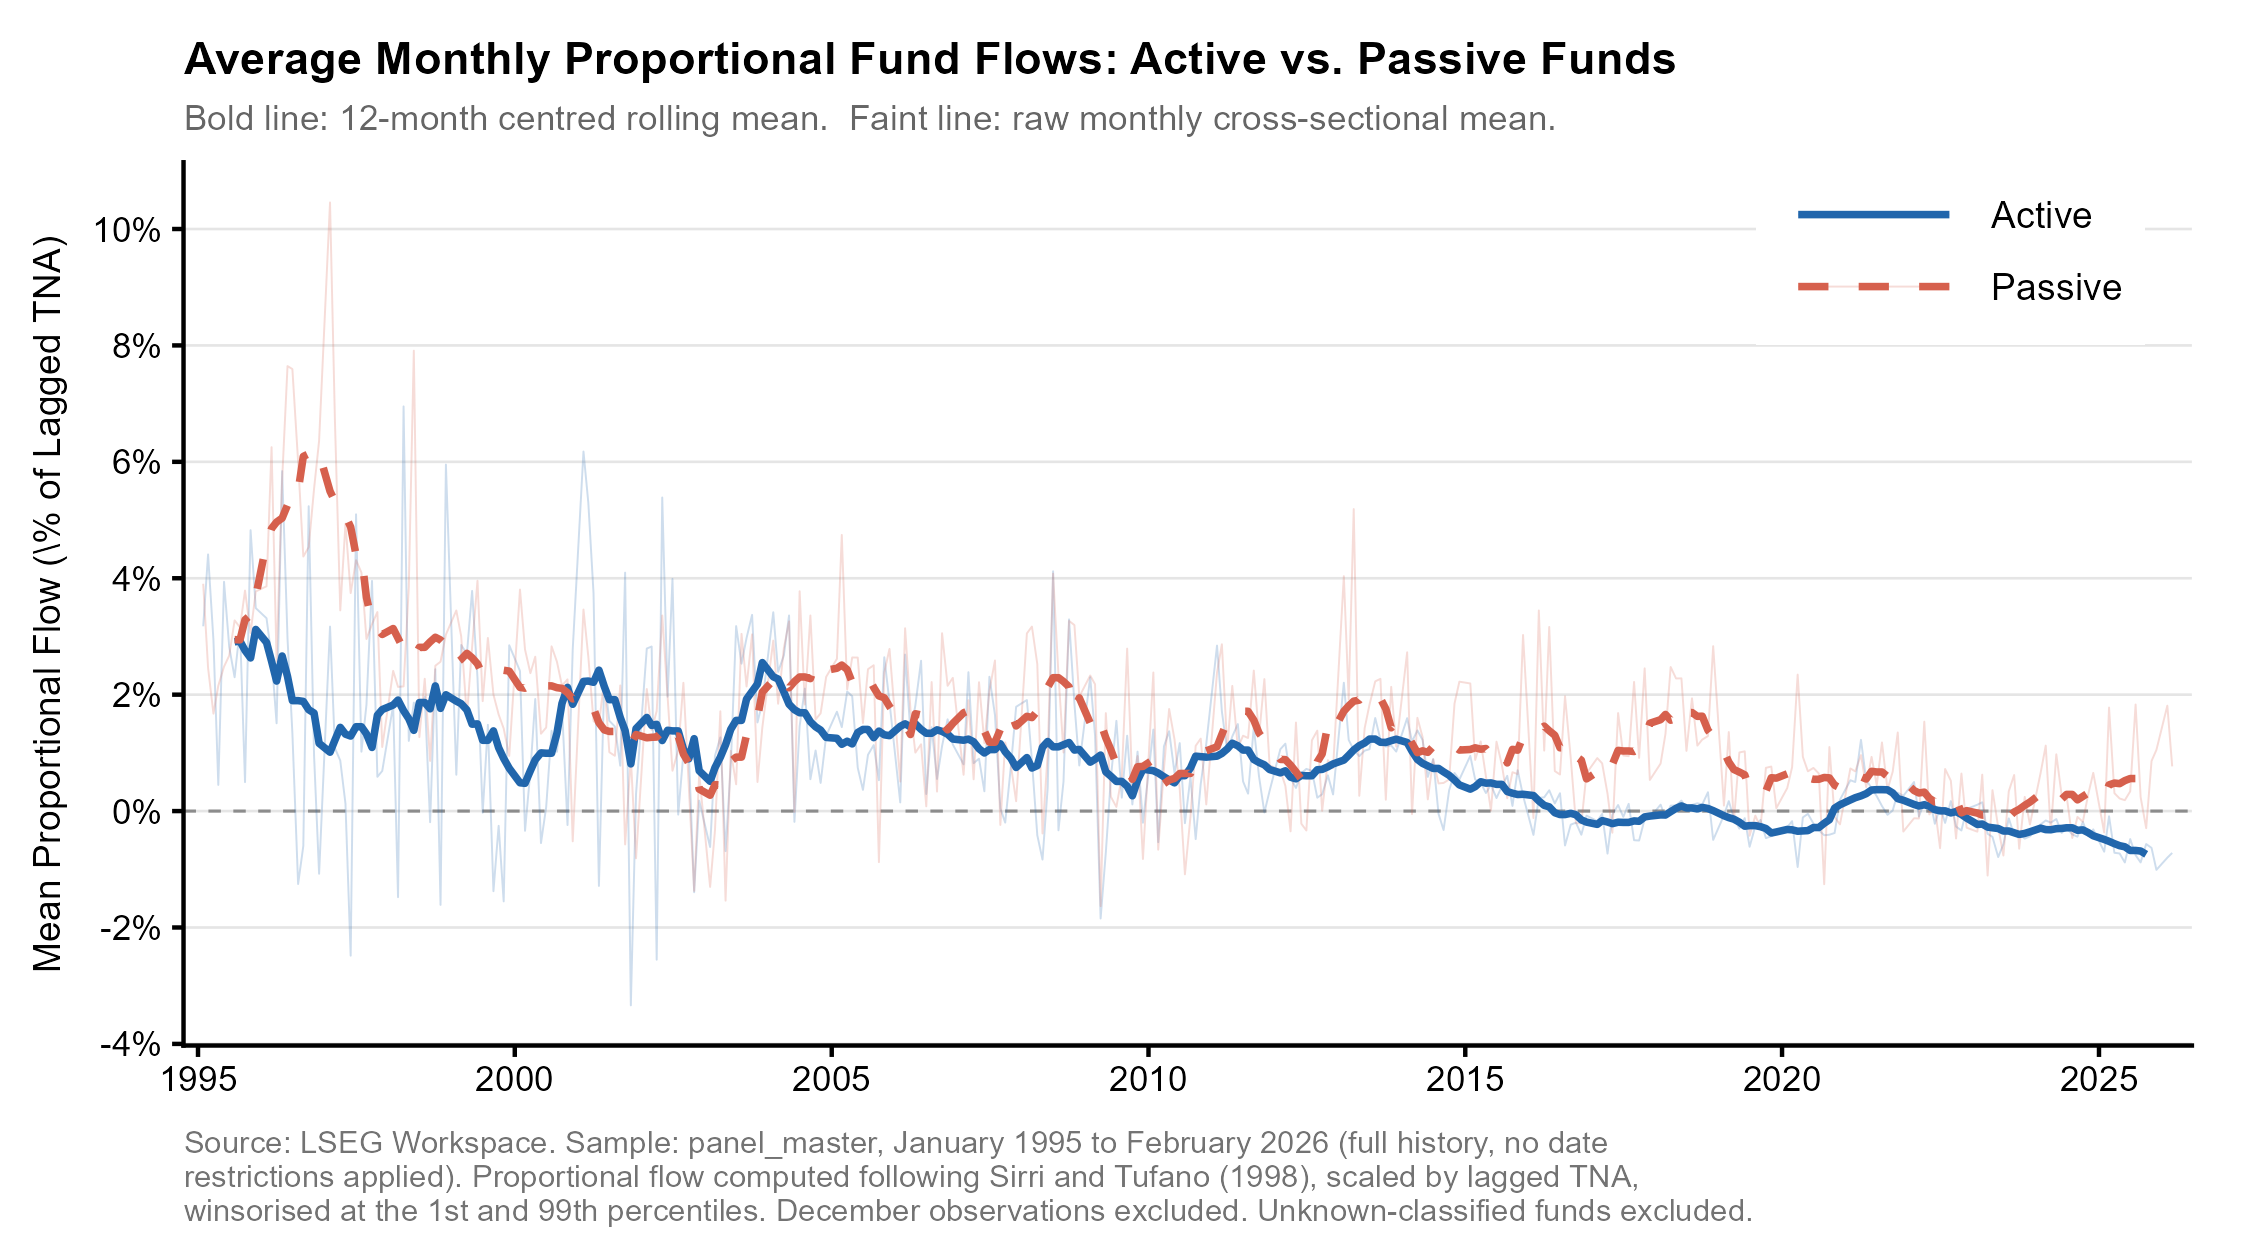
\includegraphics[width=\linewidth]{tables/fig_fund_flows}}{%
        \fbox{\parbox[c][4cm][c]{\linewidth}{\centering\footnotesize\texttt{fig\_fund\_flows.png}}}}
    \end{column}
    \begin{column}{0.38\textwidth}
      \begin{itemize}\itemsep5pt
        \item Average monthly proportional fund flows: active vs.\ passive.
        \item Passive flows persistently above active post-2010.
        \item Active flows declined structurally after the 2011 break.
        \item Flow convexity (winner-chasing) visible as spikes in active flows
              around return peaks.
      \end{itemize}
    \end{column}
  \end{columns}
\end{frame}

\end{document}
